% !TEX root = ../main.tex

\section{Dataset Overview}
\label{schema}

The steps in Section~\ref{dataset} led to the construction of the 
Wonderless Serverless computing dataset, consisting of 1,877
real-world Serverless applications worthing 44 GB of data. 
The dataset is available in the two following formats.

First, a CSV file that contains the URL of each repository. 
With this format one can clone the latest version of the repositories at any time; 
However, the repositories can change access to private, 
be removed entirely, or drop the services related to Serverless computing 
over time. 

To overcome these issues, we provide a snapshot of the 
repositories taken on November 8, 2020. 
In the snapshot, each repository is assigned a directory named `$a\_b$' 
where `$a$' is the GitHub username of the developer and `$b$' is the name of the repository. 
The directories are categorized into seven groups based on the provider of the application, 
retrieved from the $serverless.yml$ configuration file. 
The categories are \emph{AWS}, \emph{Azure}, \emph{Google}, \emph{OpenWhisk}, 
\emph{Cloudflare}, \emph{Kubeless}, 
and \emph{Other}. The \emph{Other} category contains providers supporting less than three 
applications in the dataset. If an application used multiple providers, we placed the repository in 
all the related groups. 

Wonderless comprises 197,993 files developed in various programming languages. 
Other than Serverless services, an application can have non-Serverless parts 
developed in different programming languages. We define the runtime of a 
Serverless application based on the runtime specified in the configuration file of that application.
We used CLOC\footnote{\url{https://github.com/AlDanial/cloc}} to count the number of files and 
lines of code for each language. Table~\ref{tab:pl} presents an overview, 
including the occurrence of the runtimes in the dataset. 
% Based on the applications in the dataset, 
Node.js, with 72.2\% occurrences in Wonderless, is the most popular runtime.
%for Serverless applications 

\begin{table}[h]
	\begin{center}
		\caption{Distribution of programming languages in Wonderless.}
		\label{tab:pl}
		\begin{tabular}{c|c|c|c}
			\textbf{Language} & \textbf{Files} & \textbf{Lines of Code} & \textbf{Occurrence\%} \\
			\toprule
			JavaScript &  44,279 & 7,332,365 & \multirow{2}{*}{72.2\%} \\
			TypeScript & 22,517 & 1,429,896 &  \\ \midrule
			Python & 15,875 & 2,083,442 & 19\% \\ \midrule
			Java & 11,556 & 415,665 & 2.7\%  \\ \midrule
			Ruby & 3,001 & 91,499 & 0.5\%  \\ \midrule
			Go & 2,283 & 489,636 & 2.4\% \\ \midrule
			Other & 98,482 & 28,281,135 & 3.2\% \\ \midrule
			Total & 197,993 & 40,123,638 & 100\% \\ \midrule
		\end{tabular}
	\end{center}
\vspace{-7mm}
\end{table}

Wonderless includes the Git history of each repository. 
According to the results from \emph{git log}, there are 374,922 commits in total, 
and 13,984 developers contributed to these applications.
More than 48\% of the repositories have at least one 
GitHub star, and more than 96\% have less than 100 stars.
%%
%\begin{figure}
%	\centering
%	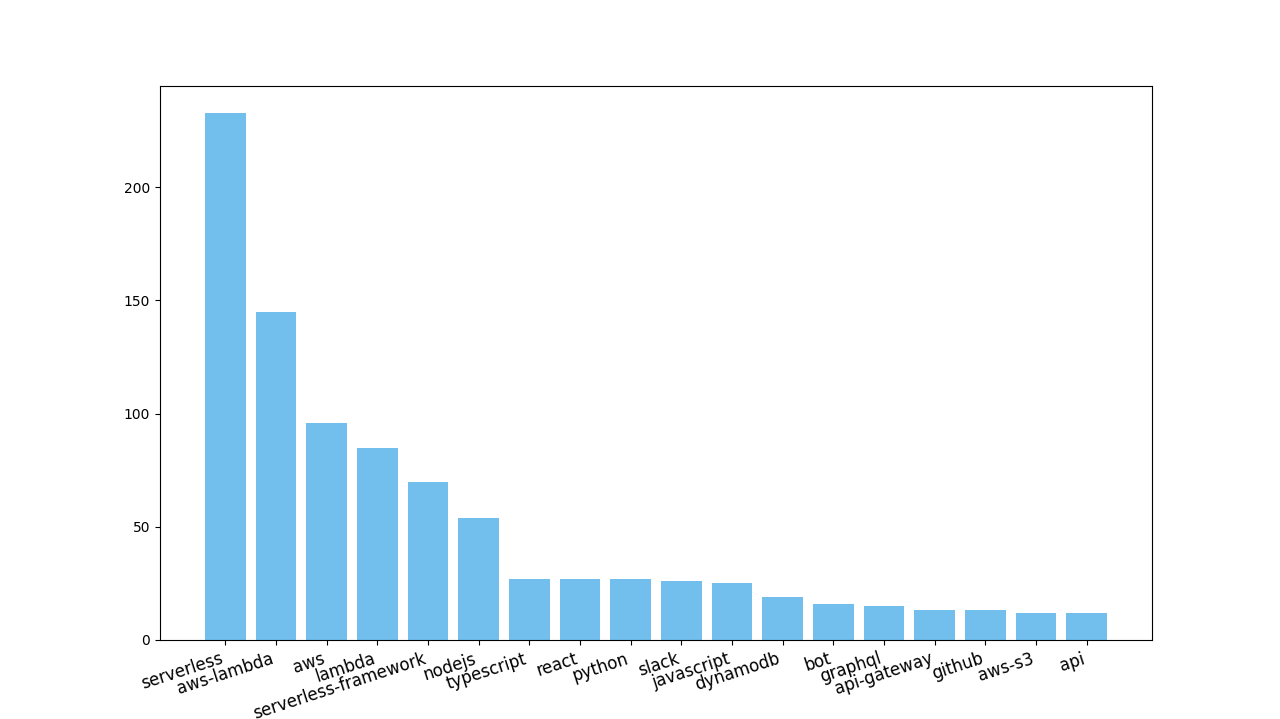
\includegraphics[scale=0.3]{figures/topics.png}
%	\caption{Popular topics in Serverless applications.}
%	\label{fig:topics}
%\end{figure}
%%
%More than $\%80$ of the applications have less than five contributors.
%%
%We extracted the meta-data of repositories using the \emph{mercy-preview} media 
%type of GitHub API previews. Based on this data, $\%46$ of the repositories have a license 
%among which $\%67$ are MIT License. Figure~\ref{fig:topics} 
%represents the distribution of topics with more than ten occurrences in the dataset.



